%% chapters/behavior_modeling/ch1_rut.tex
%% 第1章　ランダム効用最大化理論の基礎
\section{ランダム効用最大化理論}\label{sec:rut}

本節では行動モデルの理解にあたり，ランダム効用最大化理論（Random Utility Maximization Theory, RUM）\cite{mcfadden1977modelling}を導入する．
本教科書で扱う範囲ではより厳密には加法的ランダム効用最大化理論（Additive Random Utility Maximization Theory, ARUM）と呼ぶべきものであるが，以下では便宜上RUMと呼ぶことにする．
RUM はミクロ経済学の重要な仮定であり，個人は効用を最大化するような合理的な選択行動を行うとするものである．

本節の構成は以下の通りである．
まず\ref{ssec:utility_random}項で効用関数の記述と誤差項の導入を行い，\ref{ssec:iid_assumption}項で誤差項の独立同一性の仮定を述べる．
続いて\ref{ssec:error_distribution}項で誤差項の分布形状（正規分布・ガンベル分布）を具体的に示し，多項ロジット（MNL）モデルを導出する．
最後に\ref{ssec:iia_intro}項で，MNLモデルが持つIIA特性の問題と，次節以降での拡張への動機を述べる．

\subsection{効用の記述とランダム性の導入}\label{ssec:utility_random}
まず選択肢の効用評価の記述方法を述べる．
各選択肢 $a$ は分析者によって設定された説明変数 $x_{i}$ および対応するパラメータ $\beta_{i}$ を用いて評価される．
その評価関数を効用関数と呼び，通常は線形な形式で表される．
すなわち，選択肢 $a$ の効用 $U_{a}$ は以下のように表される．
\begin{equation}\label{eq:utility_func_det}
U_{a} = \sum_{i} \beta_{i} x_{i}
\end{equation}
なお本定式化では個人の異質性は考慮していない．
例えば交通手段選択であれば，説明変数 $\bm{x}$ は「旅行時間」「旅行費用」「快適さ」などの属性を表し，パラメータ $\bm{\beta}$ はこれらの属性が効用に与える影響の大きさを表す．
行動モデルの目的は，この効用関数を用いて個人の選択行動を記述することであり，それは各パタメータ $\beta_{i}$ を推定することに帰着する．

個人 $k$ の選択行動結果を $y_k$ と表すと，効用最大化の仮定により
\begin{equation}\label{eq:utility_max}
y_k = \argmax_{a} U_{a}
\end{equation}
となる．
これは毎回確定的な選択が行われることを示すが，実際にはこのように確定的に対象の選択行動を説明することは困難である．
なぜなら，\eqref{eq:utility_func_det}は各選択肢が分析者によって選定された特定の説明変数 $\bm{x}$ に基づいて評価されることを前提としているが，真の効用関数は選択者毎の私的情報そのものであり，分析者が全ての構成を把握することは原理的に困難であるためである．
このような不確実性を考慮するために，効用関数\eqref{eq:utility_func_det}にランダム性を加えるための誤差項 $\varepsilon_a$ を導入する．
すなわち，選択肢 $a$ の効用は以下のように再定義される．
\begin{equation}\label{eq:utility_func_random}
U_{a} = \sum_{i} \beta_{i} x_{a, i} + \varepsilon_a
\end{equation}
$\varepsilon_a$ は選択肢 $a$ に特有のランダムな誤差項であり，上で述べた個人の選択行動に影響を与えるが分析者が観測できない要因を表す．
なおこの誤差項に対し，従来の確定的な効用項 $V_a = \sum_i \beta_i x_{a, i}$ を確定項と呼ぶ．


\subsection{誤差項の独立同一性の仮定}\label{ssec:iid_assumption}
本項及び次項では誤差項に関する具体的な仮定を導入する．

まず，誤差項の独立同一性（Independent Identical Distribution, i.i.d.）に関する仮定を導入する．

効用関数\eqref{eq:utility_func_det}は最も一般的には個人 $k$ ，選択肢 $a$ に依存する値として表される．
\begin{equation}
U_{ka} = V_{ka} + \varepsilon_{ka}
\end{equation}

\textbf{独立同一性: Independent and Identically Distributed (i.i.d.)}は以下の二つの要素からなる．
\begin{description}
  \item[独立性] 各個人および選択肢の組 $k, a$ に対して $\varepsilon_{ka}$ は互いに独立である．
  \item[同一分布] 各個人および各選択肢の組 $k, a$ に対して $\varepsilon_{ka}$ は同一の確率分布に従う．
\end{description}
ここで独立とは，ある選択肢に関する未観測要因が他の選択肢の未観測要因と相関を持たないことを意味し，同一分布とは，それらの未観測要因のばらつき方がすべての選択肢・個人で同じであることを意味する．

\subsection{誤差項の分布形状}\label{ssec:error_distribution}
続いて誤差項の分布形状を考える．
誤差項によるランダム性の導入に伴い，\eqref{eq:utility_max}は次のように書き換えられる（個人 $k$ の識別子は省略）．
\begin{equation}\label{eq:utility_max_random}
y_k = \argmax_{a} \left( \sum_{i} \beta_{i} x_{a, i} + \varepsilon_a \right) = \argmax_{a} \left( V_a + \varepsilon_a \right)
\end{equation}
選択肢 $a$ の選択確率は次のように表される．
\begin{equation}\label{eq:choice_prob}
  \begin{aligned}
    \text{Pr}(y_k = a) &= \text{Pr}\left( V_a + \varepsilon_a > V_{a'} + \varepsilon_{a'} \quad \forall a' \neq a \right) \\
    &= \text{Pr}\left( V_a - V_{a'} > \varepsilon_{a'} - \varepsilon_a \quad \forall a' \neq a \right) \\
    &= \text{Pr}_{\varepsilon}\left( V_a - V_{a'} > \varepsilon \quad \forall a' \neq a \right) \\
    &= \int_{-\infty}^{V_a - V_{a'}} f(\varepsilon) d\varepsilon \\
    &= F_{\varepsilon}(V_a - V_{a'})
  \end{aligned}
\end{equation}

従って選択確率は誤差項 $\varepsilon$ の確率分布 $f(\varepsilon)$ および累積分布関数 $F_{\varepsilon}(\varepsilon)$ に明らかに依存する．

% では続いてこの誤差項 $\varepsilon$ の分布形状を具体的に与えてみよう．
% なお以下では前項で導入した通り誤差項はi.i.d.であると仮定する．

% \subsubsection{正規分布の場合}
% 最も一般的な分布は正規分布である．
% ここで標準正規分布の確率密度関数を $\phi(\cdot)$，その累積分布関数を $\Phi(\cdot)$ と表すと，選択確率 $\text{Pr}(y_k = a)$ は次のように表される．
% \begin{equation}
%   \text{Pr}(y_k = a) = \int_{-\infty}^{V_a - V_{a'}} \phi(\varepsilon) \, d\varepsilon = \Phi(V_a - V_{a'})
% \end{equation}
% この選択確率は一般に閉じた形で表すことができないため，数値的な積分が必要となり計算コストが高い．
% なお，本モデルを \textbf{Probit Model}と呼ぶ．

では続いてこの誤差項 $\varepsilon$ の分布形状を具体的に与えてみよう．

\subsubsection{正規分布の場合}
誤差項に正規分布を仮定したものが \textbf{Probit Model} である．

まず二項選択の場合を考える．
\eqref{eq:choice_prob}において $\bm{\varepsilon}=(\varepsilon_1,\varepsilon_2)$ が2変数正規分布 $MVN(0, \Sigma)$ に従うと仮定する．
ここで，
\begin{equation}
  \Sigma = \begin{bmatrix}
    \sigma_1^2 & \sigma_{12} \\
    \sigma_{12} & \sigma_2^2
  \end{bmatrix}
\end{equation}
である．
分散共分散行列 $\Sigma$ の非対角成分は選択肢間の誤差相関を表すが，これによって相関を許容できる点が Probit Model の利点の一つである．

$\varepsilon_2-\varepsilon_1$ は$\sigma^2=\mathrm{Var}(\varepsilon_2-\varepsilon_1)$ の分散を持つ正規分布 $N(0,\sigma^2)$ に従うため，
\begin{equation}
  P_1 = \Phi\!\left(\frac{V_1-V_2}{\sigma}\right)
\end{equation}
を得る．
このように二項選択の場合は closed-form で表されるため，数値的な積分を必要とせず計算が容易である．

一方，多項の場合の選択確率は一般に多変量正規分布の積分として表されるため，二項の場合と異なり closed-form で簡潔に表せないことが多い．
そのため実際の推定には数値積分やシミュレーションが必要となり，計算コストが高くなる．

\subsubsection{ガンベル分布の場合}
これに対して，誤差項が先述したi.i.d.なガンベル分布に従うと仮定したものが\textbf{Logit Model} である．
ガンベル分布は正規分布と類似の形状を持つが，累積分布関数がclosed-formで表されるという特徴がある．
ガンベル分布の累積分布関数は次のように表される．
\begin{equation}\label{eq:gumbel_cdf}
  F(x) = \exp\bigl(-\exp(-\mu (x - \eta))\bigr)
\end{equation}
ここで $\eta$ はロケーションパラメータ（分布の最頻値に一致），$\mu > 0$ はスケールパラメータ（分布のばらつきに関係）である．
離散選択モデルにおいては，通常 $\eta = 0$，$\mu = 1$ に正規化する．
ロケーションパラメータ $\eta$ は効用の確定項 $V_a$ に吸収でき，スケールパラメータ $\mu$ はパラメータ $\beta_i$ と同時には識別できない（$\mu V_a = \mu \sum_i \beta_i x_{a,i}$ より，推定されるのは常に $\mu \beta_i$ の積である）ためである．

この正規化のもとで，選択確率は次のように表される．
\begin{equation}
  \text{Pr}(y_k = a) = \frac{\exp(V_a)}{\sum_{a'} \exp(V_{a'})}
\end{equation}

これはclosed-formで表されるため，数値的な積分を必要とせず計算が容易である．
従って離散選択モデルにおいてはガンベル分布を使用することが多い．

一般に行動モデルの文脈で離散選択モデルを用いる際には，上記仮定を踏まえて誤差項に i.i.d. ガンベル分布を仮定することが多い．
すなわち効用関数を以下のように宣言することが多い． 
\begin{equation}
U_{ka} = V_{ka} + \varepsilon_{ka}, \quad \varepsilon_{ka} \sim \text{i.i.d. Gumbel}
\end{equation}

なお選択肢が二つの場合は特に Binary Logit Model と呼び，複数の場合は \textbf{Multinomial Logit Model} と呼ぶ．

\subsubsection{摂動効用理論との関連}
なお序章で述べたように，Logit 選択確率は摂動効用理論の観点からも導出できる．
具体的には，需要ベクトル $p$（各選択肢の選択確率）に対して，
期待効用に Shannon entropy による正則化項を加えた
\begin{equation}\label{eq:perturbed_utility}
\max_{p_a\ge 0,\ \sum_a p_a=1}
\left\{
\sum_a p_a V_a + \mu H(p)
\right\},
\qquad
H(p)=-\sum_a p_a \ln p_a
\tag{3.11}
\end{equation}
を考えると，その最適解として Logit 選択確率が得られる．
ここで，しばしば
\begin{equation}\label{eq:corrected_entropy}
  H(p)=-\sum_a (p_a\ln p_a-p_a)
\end{equation}
と等価に書かれることもあるが，これは制約 $\sum_a p_a=1$ のもとで定数差しか持たず，最適解には影響しない．

このことは，ARUM において「誤差項に i.i.d. Gumbel 分布を仮定する」ことと，
摂動効用理論において「Shannon entropy 型の正則化項を導入する」ことが，
同一の Logit 選択確率を与える等価な表現であることを意味する．
すなわち，一方は誤差項の分布仮定によって，他方は摂動項の形状によって，
同じ行動仮説を表現していると解釈できる．
この双対的な見方は，第3節で摂動効用理論に基づく経路選択モデルを導入する際に重要となる．

なお，ガンベル分布と正規分布の確率密度関数は図\ref{fig:gumbel-pdf}のような形状をしている．
\begin{figure}[hbtp]
  \centering
    \resizebox{.9\linewidth}{!}{%
      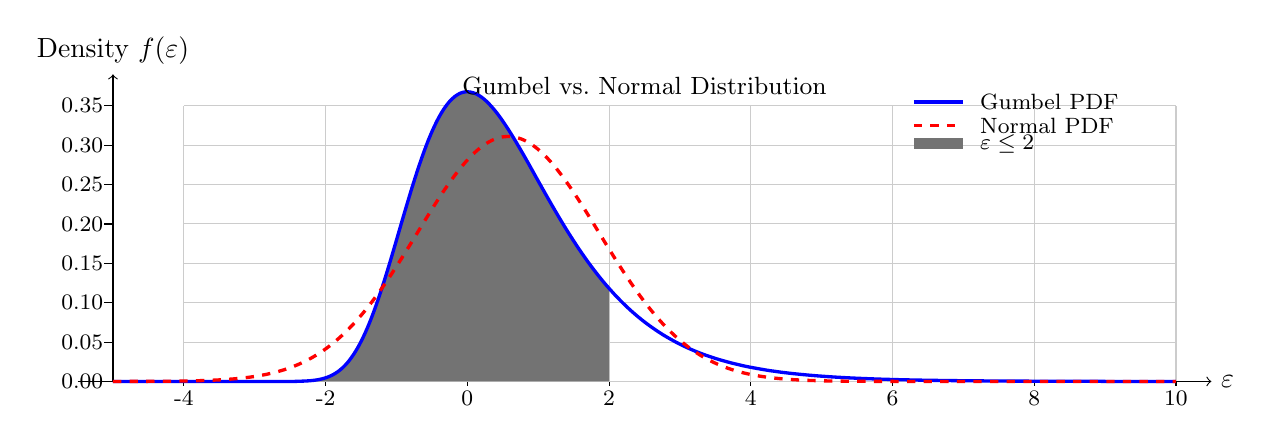
\begin{tikzpicture}[x=0.9cm,y=10cm]
  % axes
  \draw[->] (-5.5,0) -- (10.5,0) node[right] {$\varepsilon$};
  \draw[->] (-5,0) -- (-5,0.39) node[above] {Density $f(\varepsilon)$};

  % x ticks
  \foreach \x in {-4,-2,0,2,4,6,8,10}{
    \draw (\x,0) -- (\x,-0.006);
    \node[below,font=\footnotesize] at (\x,0) {\x};
  }

  % y ticks
  \foreach \y in {0.00,0.05,0.10,0.15,0.20,0.25,0.30,0.35}{
    \draw (-5,\y) -- (-5.12,\y);
    \node[left,font=\footnotesize] at (-5,\y) {\y};
  }

  % grid
  \draw[gray!40, thin] (-4,0) grid[xstep=2,ystep=0.05] (10,0.35);

  % shaded area
  \fill[black!55]
    plot[smooth,domain=-5:2,samples=120]
      (\x,{exp(-(\x + exp(-\x)))})
    -- (2,0) -- (-5,0) -- cycle;

  % Gumbel curve
  \draw[blue, very thick]
    plot[smooth,domain=-5:10,samples=200]
      (\x,{exp(-(\x + exp(-\x)))});

  % Normal distribution (mu=0.5772, sigma=pi/sqrt(6)=1.2826) to match Gumbel mean & variance
  \draw[red, very thick, dashed]
    plot[smooth,domain=-5:10,samples=200]
      (\x,{exp(-0.5*((\x - 0.5772)/1.2826)^2) / (1.2826*2.5066)});

  % title
  \node[font=\small] at (2.5,0.375)
    {Gumbel vs.\ Normal Distribution};

  % legend
  \draw[blue, very thick] (6.3,0.355) -- (7.0,0.355);
  \node[right,font=\footnotesize] at (7.1,0.355) {Gumbel PDF};

  \draw[red, very thick, dashed] (6.3,0.325) -- (7.0,0.325);
  \node[right,font=\footnotesize] at (7.1,0.325) {Normal PDF};

  \fill[black!55] (6.3,0.295) rectangle (7.0,0.309);
  \node[right,font=\footnotesize] at (7.1,0.302) {$\varepsilon \le 2$};
\end{tikzpicture}%
    }
  \caption{ガンベル分布の確率密度関数(PDF)と，$\varepsilon \le 2$ の領域}
  \label{fig:gumbel-pdf}
\end{figure}


\subsection{選択肢・個人間の相関・異質性の扱いとIIA性の問題}\label{ssec:iia_intro}
上記では誤差項の独立同一性（i.i.d.）に関する仮定を導入したが，この仮定は現実の選択行動を記述する上でしばしば問題となる．
例えば交通行動の文脈においては，互いに類似した交通手段や重複区間の多い経路どうしで未観測効用が似通うことが多く，独立性の仮定がしばしば問題となる．
また隣接する複数の地点は，距離が離れた地点と比べて特徴が似通うことが多いため，目的地選択の文脈においても独立性の仮定が問題となる．
さらに時間価値や混雑回避傾向は個人によって異なるため，個人間で同一の分布を仮定することも強い制約となる．
こうした理由から，Nested Logit や Mixed Logit など，i.i.d. 仮定を緩和するモデルが導入されてきた．
これらのモデルについては次節にて詳述する．
